
\documentclass[]{article}
\voffset=-1.5cm
\oddsidemargin=0.0cm
\textwidth = 480pt

% http://www.strath.ac.uk/aer/materials/5furtherquantitativeresearchdesignandanalysis/unit6/whatislogisticregression/

% http://www.medcalc.org/manual/logistic_regression.php


\usepackage{amsmath}
\usepackage{graphicx}
\usepackage{amssymb}
\usepackage{framed}
\usepackage{multicol}
%\usepackage[paperwidth=21cm, paperheight=29.8cm]{geometry}
%\usepackage[angle=0,scale=1,color=black,hshift=-0.4cm,vshift=15cm]{background}
%\usepackage{multirow}
\usepackage{enumerate}


\begin{document}
	
\section*{Lab 2 Part B : One-Sample T-Test using SPSS Statistics}

\section{Introduction}
\begin{itemize}
	\item The one-sample t-test is used to determine whether a sample comes from a population with a specific mean. This population mean is not always known, but is sometimes hypothesized. 
\item For example, you want to show that a new teaching method for pupils struggling to learn English grammar can improve their grammar skills to the national average. Your sample would be pupils who received the new teaching method and your population mean would be the national average score. 
\item Alternately, you believe that doctors that work in Accident and Emergency (A \& E) departments work 100 hour per week despite the dangers (e.g., tiredness) of working such long hours. You sample 1000 doctors in A \& E departments and see if their hours differ from 100 hours.
	
\item This guide shows you how to carry out a one-sample t-test using SPSS Statistics, as well as interpret and report the results from this test. \item However, before we introduce you to this procedure, you need to understand the different assumptions that your data must meet in order for a one-sample t-test to give you a valid result. We discuss these assumptions later in the appendix.
\end{itemize}


%============================================%

\section{Implementation}
In the section,  we illustrate the SPSS Statistics procedure required to perform a one-sample t-test assuming that no assumptions have been violated. First, we set out the example we use to explain the one-sample t-test procedure in SPSS Statistics.

%============================================%


%============================================%
\subsection{Example and Setup in SPSS Statistics}
\begin{itemize}
	\item A researcher is planning a psychological intervention study, but before he proceeds he wants to characterise his participants' depression levels.
\item He tests each participant on a particular depression index, where anyone who achieves a score of 4.0 is deemed to have 'normal' levels of depression. Lower scores indicate less depression and higher scores indicate greater depression.
\item  He has recruited 40 participants to take part in the study. Depression scores are recorded in the variable \texttt{dep\_score}. 
\item He wants to know whether his sample is representative of the normal population (i.e., do they score statistically significantly differently from 4.0).
	
\item For a one-sample t-test, there will only be one variable's data to be entered into SPSS Statistics: the dependent variable, \texttt{dep\_score}, which is the depression score.
\end{itemize}


%============================================%
\subsection{Test Procedure in SPSS Statistics}
\begin{itemize}
	\item The five steps below show you how to analyse your data using a one-sample t-test in SPSS Statistics when the four relevant assumptions have not been violated (see Appendix). 
	
\item At the end of these five steps, we show you how to interpret the results from this test. 
%If you are looking for help to make sure your data meets assumptions No. 3 and No. 4, which are required when using a one-sample t-test, and can be tested using SPSS Statistics, you can learn more in our enhanced guides here.
\end{itemize}


\noindent \textbf{Step 1:} Click \textbf{Analyze $>$ Compare Means $>$ One-Sample T Test}... on the main menu:


\begin{figure}[h!]
\centering
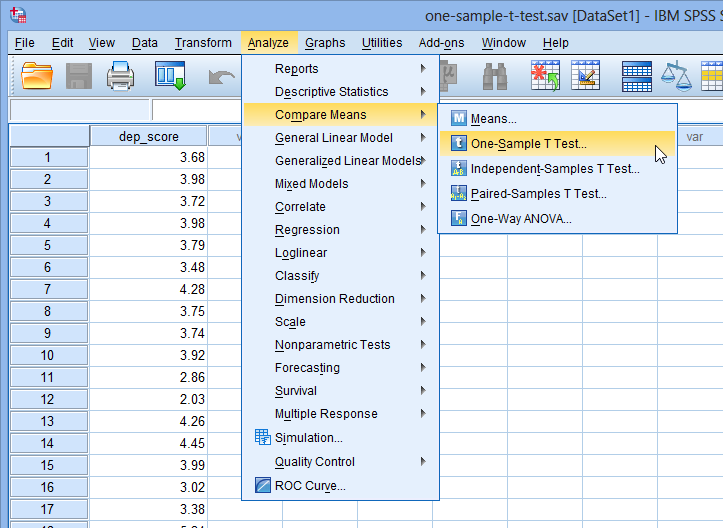
\includegraphics[width=0.45\linewidth]{OneSample/OneSample1}

\label{fig:OneSample1}
\end{figure}

\noindent You will be presented with the One-Sample T Test dialogue box, as shown below:


\begin{figure}[h!]
	\centering
	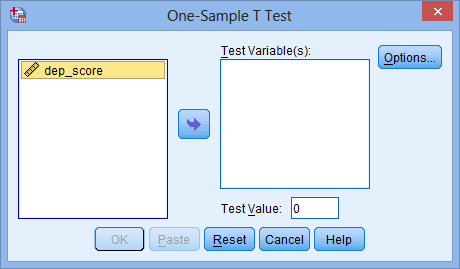
\includegraphics[width=0.5\linewidth]{OneSample/OneSample2}
	\label{fig:OneSample2}
\end{figure}
\newpage
\noindent Transfer the dependent variable, \texttt{dep\_score}, into the \texttt{Test Variable(s):} box by selecting it (by clicking on it) and then clicking on the  button.  \smallskip

\begin{itemize}
	\item \noindent Enter the population mean you are comparing the sample against in the\texttt{ Test Value:} box, by changing the current value of ``0" to ``4". You will end up with the following screen:
\end{itemize}



\begin{figure}[h!]
	\centering
	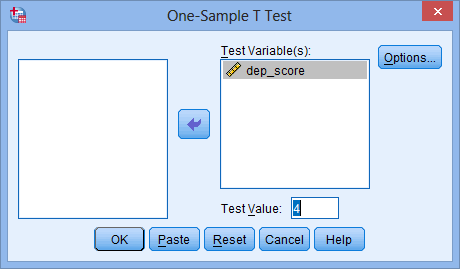
\includegraphics[width=0.5\linewidth]{OneSample/OneSample3}
	\label{fig:OneSample3}
\end{figure}
\begin{itemize}
	\item Click on the \texttt{Options} button. You will be presented with the\texttt{ One-Sample T Test: Options} dialogue box, as shown below:
\end{itemize}



\begin{figure}[h!]
	\centering
	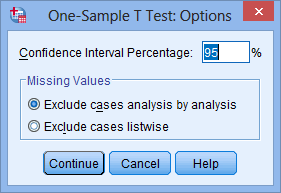
\includegraphics[width=0.5\linewidth]{OneSample/OneSample4}

	\label{fig:OneSample4}
\end{figure} \medskip
\noindent For this example, keep the default 95\% confidence intervals and Exclude cases analysis by analysis in the –Missing Values– area.
\newpage
\begin{framed}
\noindent \textit{Note 1:\\ By default, SPSS Statistics uses 95\% confidence intervals (labelled as the Confidence Interval Percentage in SPSS Statistics). This equates to declaring statistical significance at the $p < .05$ level. }
	
\textit{If you wish to change this you can enter any value from 1 to 99. For example, entering "99" into this box would result in a 99\% confidence interval and equate to declaring statistical significance at the $p < .01$ level. For this example, keep the default 95\% confidence intervals.}
\end{framed}
\begin{framed}
\noindent \textit{Note 2:\\ If you are testing more than one dependent variable and you have any missing values in your data, you need to think carefully about whether to select Exclude cases analysis by analysis or Exclude cases listwise) in the –Missing Values– area. Selecting the incorrect option could mean that SPSS Statistics removes data from your analysis that you wanted to include.}
% We discuss this further and what options to select in our enhanced one-sample t-test guide.}
\end{framed}

\begin{itemize}
	\item Click the \texttt{continue} button. You will be returned to the One-Sample T Test dialogue box. Then click the \texttt{OK} button to generate the output.
\end{itemize}




%============================================% 
%============================================%
\subsection{Interpreting the SPSS Statistics output of the one-sample t-test}
SPSS Statistics generates two main tables of output for the one-sample t-test that contains all the information you require to interpret the results of a one-sample t-test.
\begin{itemize}
	\item If your data passed assumption No. 3 (i.e., there were no significant outliers) and assumption No. 4 (i.e., your dependent variable was approximately normally distributed for each category of the independent variable), which we explained earlier in the Assumptions section, you will only need to interpret these two main tables. 
	\item However, since you should have tested your data for these assumptions, you will also need to interpret the SPSS Statistics output that was produced when you tested for them (i.e., you will have to interpret: (a) the boxplots you used to check if there were any significant outliers; and (b) the output SPSS Statistics produces for your Shapiro-Wilk test of normality to determine normality). 
	%If you do not know how to do this, we show you in our enhanced one-sample t-test guide. 
	\item Remember that if your data failed any of these assumptions, the output that you get from the one-sample t-test procedure (i.e., the tables we discuss below), will no longer be relevant, and you will need to interpret these tables differently.
\end{itemize}


However, in this guide, we take you through each of the two main tables in turn, assuming that your data met all the relevant assumptions:

\newpage
\section{Descriptive statistics}
You can make an initial interpretation of the data using the One-Sample Statistics table, which presents relevant descriptive statistics:

\begin{figure}[h!]
\centering
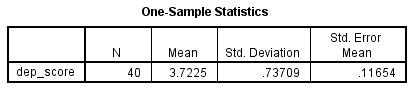
\includegraphics[width=0.7\linewidth]{OneSample/OneSample-DescriptiveStatistics1}
\label{fig:OneSample-DescriptiveStatistics1}
\end{figure}

It is more common than not to present your descriptive statistics using the mean and standard deviation (``\texttt{Std. Deviation}" column) rather than the standard error of the mean ("\texttt{Std. Error Mean}" column), although both are acceptable. 



\begin{framed}
You could report the results, using the standard deviation, as follows:

Mean depression score ($3.72 \pm 0.74$) was lower than the population 'normal' depression score of 4.0.
\end{framed}
\begin{itemize}
\item However, by running a one-sample t-test, you are really interested in knowing whether the sample you have (\texttt{dep\_score}) comes from a 'normal' population (which has a mean of 4.0). This is discussed in the next section.
\end{itemize}
\subsection{One-sample t-test}
The One-Sample Test table reports the result of the one-sample t-test. The top row provides the value of the known or hypothesized population mean you are comparing your sample data to, as highlighted below:


\begin{figure}[h!]
	\centering
	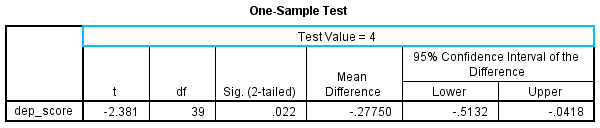
\includegraphics[width=0.7\linewidth]{OneSample/OneSample-DescriptiveStatistics2}
	\caption{}
	\label{fig:OneSample-DescriptiveStatistics2}
\end{figure}
\begin{itemize}
	\item In this example, you can see the 'normal' depression score value of "4" that you entered in earlier. You now need to consult the first three columns of the One-Sample Test table, which provides information on whether the sample is from a population with a mean of 4 (i.e., are the means statistically significantly different), as highlighted below:


\begin{figure}[h!]
	\centering
	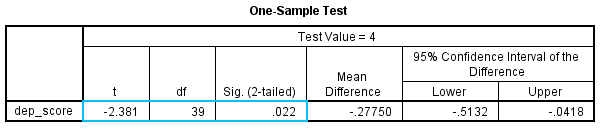
\includegraphics[width=0.7\linewidth]{OneSample/OneSample-DescriptiveStatistics3}
	\caption{}
	\label{fig:OneSample-DescriptiveStatistics3}
\end{figure}
\item Moving from left-to-right, you are presented with the observed t-value ("\texttt{t}" column), the degrees of freedom ("\texttt{df}"), and the statistical significance (p-value) ("Sig. (2-tailed)") of the one-sample t-test. 
\item In this example, $p < .05$ (it is \texttt{p = .022}). Therefore, it can be concluded that the population means are statistically significantly different. 
\item If \texttt{p > .05}, the difference between the sample-estimated population mean and the comparison population mean would not be statistically significantly different.

\item Note: If you see SPSS Statistics state that the "\texttt{Sig. (2-tailed)}" value is ".000", this actually means that $p < .0005$. It does not mean that the significance level is actually zero.

%============================================% 
\item SPSS Statistics also reports that \texttt{t = -2.381} ("t" column) and that there are 39 degrees of freedom ("\texttt{df}" column). You need to know these values in order to report your results, which you could do as follows:
\end{itemize}

\begin{framed}

Depression score was statistically significantly lower than the population normal depression score, t(39) = -2.381, p = .022.



\end{framed}
The breakdown of the last part (i.e., t(39) = -2.381, p = .022) is as follows:

\begin{figure}
\centering
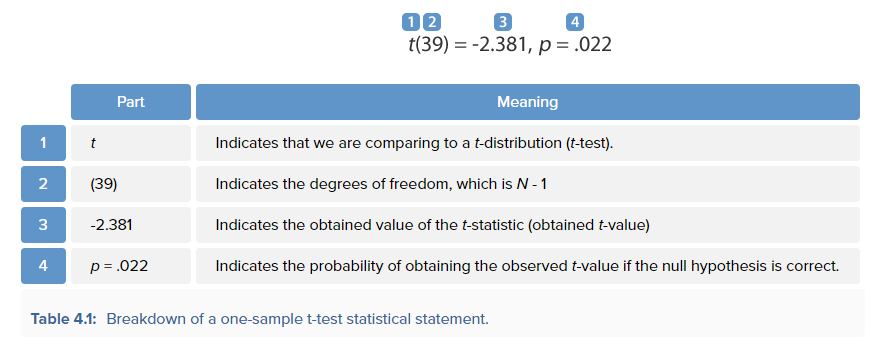
\includegraphics[width=0.7\linewidth]{OneSample/OneSample-DescriptiveStatistics4}
\label{fig:OneSample-DescriptiveStatistics4}
\end{figure}

Table 4.1:Breakdown of a one-sample t-test statistical statement.
You can also include measures of the difference between the two population means in your written report. This information is included in the columns on the far-right of the One-Sample Test table, as highlighted below:


\begin{figure}
\centering
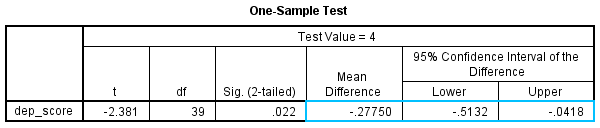
\includegraphics[width=0.7\linewidth]{OneSample/OneSample-DescriptiveStatistics5}
\label{fig:OneSample-DescriptiveStatistics5}
\end{figure}

This section of the table shows that the mean difference in the population means is -0.28 ("Mean Difference" column) and the 95\% confidence intervals (95\% CI) of the difference are -0.51 to -0.04 ("Lower" to "Upper" columns). For the measures used, it will be sufficient to report the values to 2 decimal places. You could write these results as:

\begin{framed}
\noindent Depression score was statistically significantly lower by 0.26 (95\% CI, 0.04 to 0.51) than a normal depression score of 4.0, t(39) = -2.381, p = .022.

\end{framed}
\newpage
\section{Reporting Your Results}
%============================================%
\subsection{Reporting the SPSS Statistics output of the one-sample t-test}
You can report the findings, without the tests of assumptions, as follows:
\begin{framed}
\begin{description}
\item[General]
Mean depression score (3.73 ± 0.74) was lower than the normal depression score of 4.0, a statistically significant difference of 0.26 (95\% CI, 0.04 to 0.51), t(39) = -2.381, p = .022.
\item[APA]
\end{description}
\end{framed}
Adding in the information about the statistical test you ran, including the assumptions, you have:

\begin{framed}
\noindent \textit{A one-sample t-test was run to determine whether depression score in recruited subjects was different to normal, defined as a depression score of 4.0.}
\textit{Depression scores were normally distributed, as assessed by Shapiro-Wilk's test ($p > .05$) and there were no outliers in the data, as assessed by inspection of a boxplot.}

\textit{Mean depression score (3.73 ± 0.74) was lower than the normal depression score of 4.0, a statistically significant difference of 0.26 (95\% CI, 0.04 to 0.51), t(39) = -2.381, p = .022.}
\end{framed}

Null hypothesis significance testing
You can write the result in respect of your null and alternative hypothesis as:

GeneralAPA
There was a statistically significant difference between means (p < .05) and, therefore, we can reject the null hypothesis and accept the alternative hypothesis.


%============================================%
\subsection{Practical vs. statistical significance}
\begin{itemize}
	\item Although a statistically significant difference was found between the depression scores in the recruited subjects vs. the normal depression score, it does not necessarily mean that the difference encountered, 0.26 (95\% CI, 0.04 to 0.51), is enough to be practically significant. 
	\item Indeed, the researcher might accept that although the difference is statistically significant (and would report this), the difference is not large enough to be practically significant (i.e., the subjects can be treated as normal).
	
%	\item In our enhanced one-sample t-test guide, we show you how to write up the results from your assumptions tests and one-sample t-test procedure if you need to report this in a dissertation/thesis, assignment or research report. We do this using the Harvard and APA styles. You can learn more about our enhanced content here.
\end{itemize}

\newpage
\section{Assumptions}
When you choose to analyse your data using a one-sample t-test, part of the process involves checking to make sure that the data you want to analyse can actually be analysed using a one-sample t-test. 


You need to do this because it is only appropriate to use a one-sample t-test if your data "passes" four assumptions that are required for a one-sample t-test to give you a valid result. 

In practice, checking for these four assumptions just adds a little bit more time to your analysis, requiring you to click a few more buttons in SPSS Statistics when performing your analysis, as well as think a little bit more about your data, but it is not a difficult task.

Before we introduce you to these four assumptions, do not be surprised if, when analysing your own data using SPSS Statistics, one or more of these assumptions is violated (i.e., is not met). 

This is not uncommon when working with real-world data rather than textbook examples, which often only show you how to carry out a one-sample t-test when everything goes well! However, don’t worry. Even when your data fails certain assumptions, there is often a solution to overcome this. First, let’s take a look at these four assumptions:

\begin{description}
	\item[Assumption No. 1: Correct Scale] Your dependent variable should be measured at the interval or ratio level (i.e., continuous). Examples of variables that meet this criterion include revision time (measured in hours), intelligence (measured using IQ score), exam performance (measured from 0 to 100), weight (measured in kg), and so forth. You can learn more about interval and ratio variables in our article: Types of Variable.
	
	\item[Assumption No. 2: Independence] The data are independent (i.e., not correlated/related), which means that there is no relationship between the observations. This is more of a study design issue than something you can test for, but it is an important assumption of the one-sample t-test.
	
	\item[Assumption No. 3: No Outliers] There should be no significant outliers. Outliers are data points within your data that do not follow the usual pattern (e.g., in a study of 100 students' IQ scores, where the mean score was 108 with only a small variation between students, one student had a score of 156, which is very unusual, and may even put her in the top 1\% of IQ scores globally). The problem with outliers is that they can have a negative effect on the one-sample t-test, reducing the accuracy of your results. Fortunately, when using SPSS Statistics to run a one-sample t-test on your data, you can easily detect possible outliers. 
	%%In our enhanced one-sample t-test guide, we: (a) show you how to detect outliers using SPSS Statistics; and (b) discuss some of the options you have in order to deal with outliers.
	
	\item[Assumption No. 4: Normality] Your dependent variable should be approximately normally distributed. We talk about the one-sample t-test only requiring approximately normal data because it is quite "robust" to violations of normality, meaning that the assumption can be a little violated and still provide valid results. You can test for normality using the Shapiro-Wilk test of normality, which is easily tested for using SPSS Statistics.
	%% In addition to showing you how to do this in our enhanced one-sample t-test guide, we also explain what you can do if your data fails this assumption (i.e., if it fails it more than a little bit).
\end{description}
\subsection{Checking Assmptions}
\begin{itemize}
	\item You can check assumptions No. 3 and No. 4 using SPSS Statistics. Before doing this, you should make sure that your data meets assumptions No. 1 and No. 2, although you don't need SPSS Statistics to do this. When moving on to assumptions No. 3 and No. 4, we suggest testing them in this order because it represents an order where, if a violation to the assumption is not correctable, you will no longer be able to use a one-sample t-test. 
	\item Just remember that if you do not run the statistical tests on these assumptions correctly, the results you get when running a one-sample t-test might not be valid. 
%%	\item This is why we dedicate a number of sections of our enhanced one-sample t-test guide to help you get this right. You can find out about our enhanced content here.
\end{itemize}


\end{document}